\pdfminorversion=7
\documentclass[12pt,letterpaper]{article}

\usepackage[margin=1in]{geometry}
\usepackage{newtxtext,newtxmath}
\usepackage{microtype}
\usepackage{amsmath}
\usepackage{graphicx}
\usepackage{booktabs}
\usepackage{caption}
\usepackage{subcaption}
\usepackage{float}
\usepackage{afterpage}
\usepackage{array}
\usepackage{multirow}
\usepackage{setspace}
\usepackage{titlesec}
\usepackage{enumitem}
\usepackage{fancyhdr}
\usepackage{needspace}
\usepackage{etoolbox}
\usepackage{placeins}
\usepackage{flafter}
\usepackage{xcolor}
\usepackage[hidelinks]{hyperref}
\usepackage[style=science,backend=biber,sorting=none,articletitle=true]{biblatex}
\usepackage{lineno}

\addbibresource{references.bib}
\graphicspath{{figures/}}

\setstretch{1.12}
\setlength{\parindent}{0.22in}
\setlength{\parskip}{0pt}
\captionsetup{font=small,labelfont=bf}
\titlespacing*{\section}{0pt}{2.0ex plus .4ex}{0.9ex}
\titlespacing*{\subsection}{0pt}{1.6ex plus .3ex}{0.7ex}
\titleformat{\section}{\large\bfseries}{\thesection}{0.7em}{}
\titleformat{\subsection}{\normalsize\bfseries}{\thesubsection}{0.7em}{}
\setlist[itemize]{leftmargin=1.2em,itemsep=2pt,topsep=4pt}
\pagestyle{fancy}
\setlength{\headheight}{13.6pt}
\fancyhf{}
\lhead{\small FluxCell draft manuscript}
\rhead{\small \thepage}
\renewcommand{\headrulewidth}{0.3pt}

\newcommand{\fluxcell}{FluxCell}
\newcommand{\epm}{electropermanent magnet}
\newcommand{\pending}{\textcolor{black}{pending measurement}}

\begin{document}

\begin{center}
{\LARGE \textbf{Pulse-programmed mechanical memory for Sarrus-cell robotic matter}}\\[1.1em]
{\large Alan Pham}\\[0.35em]
AO Labs, United States\\[1.0em]
\end{center}

\noindent\textbf{Opening summary.}
This draft frames \fluxcell{} as a small but unusually consequential physical-computing unit: a Sarrus-compatible cell whose geometry is changed by a short magnetic pulse and then held without continuous power. The current design locks a fixed electropermanent-magnetic cartridge, square 1018 steel pole plates, solid steel fork/tongue keepers, a one-axis proof before two-axis integration, and purchase quantities for four complete two-axis cells. The manuscript is intentionally evidence-bound. It claims a design direction, a build lock, and a measurement protocol now; measured force, energy, thermal, and cycle-life claims remain \pending{} until the one-axis proof is filmed and instrumented. The central argument is that a centimeter-scale cell with pulse-addressed memory could bridge soft robotics, mechanical computation, and show-safe kinetic environments: the same proof that makes a paper credible also makes a portfolio artifact legible for R\&D work in physical experiences.

\newpage
\linenumbers

\section{Introduction}

Robotic materials are moving away from single machines with remote actuators and toward distributed bodies whose local structure stores state, transforms motion, and computes mechanically \cite{byun2024,wangPhysicalComputing2026}. Soft robots have shown integrated bodies, embedded actuation, and autonomous operation \cite{wehner2016,wangEmbedded2023}, while magnetic materials have shown programmable shape change, haptic inputs, electropermanent latching, and low-power state retention \cite{knaian2010,mechamagnets2019,johnson2024,ntella2023}. The open opportunity is not only stronger actuation. It is a cell-level unit that can change geometry, hold state without continuous power, and tile into visible robotic surfaces.

\fluxcell{} addresses that opportunity by moving the difficult actuation question into a narrow overlap-gated magnetic circuit. Instead of asking a small magnetic actuator to pull a mechanism across a large air gap, the design holds the magnetic cartridge fixed and lets steel keepers slide deeper into or farther out of a working gap. A pulse changes the electropermanent state; the Sarrus/flexure structure supplies the gross motion; the keeper overlap controls whether the magnetic circuit assists the contracted state. This makes the first experiment concrete: build one axis, measure width change, current, temperature, hold, and release, then decide whether the mechanism earns two-axis integration.

The current purchase lock is deliberately pragmatic. Square pole plates and solid steel inserts are cleaner than stacked-key hacks, while still avoiding home cutting because supplier cut-length options set the steel dimensions. The one-axis proof uses one Alnico rod, one NdFeB rod, two square pole plates, two fork prongs, one center tongue, and one printed proof frame. The four-cell purchase quantity then supplies eight rods of each magnet type, twelve pole plates, sixteen fork prongs, and eight center tongues for four complete two-axis cells, plus spares \cite{fluxcellDesignLog2026,onlineMetals2026,allMetalsA362026,allMetals10182026}.

\section{Results}

\subsection{A fixed EPM cartridge turns the actuation problem into keeper overlap}

The locked architecture separates the magnetic cartridge from the moving carriers (Fig.~\ref{fig:cartridge}). The cartridge contains the Alnico coil element, the NdFeB bias element, and the top and bottom steel pole plates. The moving structure contributes steel keepers only: two fork prongs from one side and a center tongue from the opposite side. This matters because the large visible stroke is not produced by pulling steel across a large open gap. It is produced by changing how deeply already-nearby keeper material overlaps the magnetic working region.

\begin{figure}[H]
  \centering
  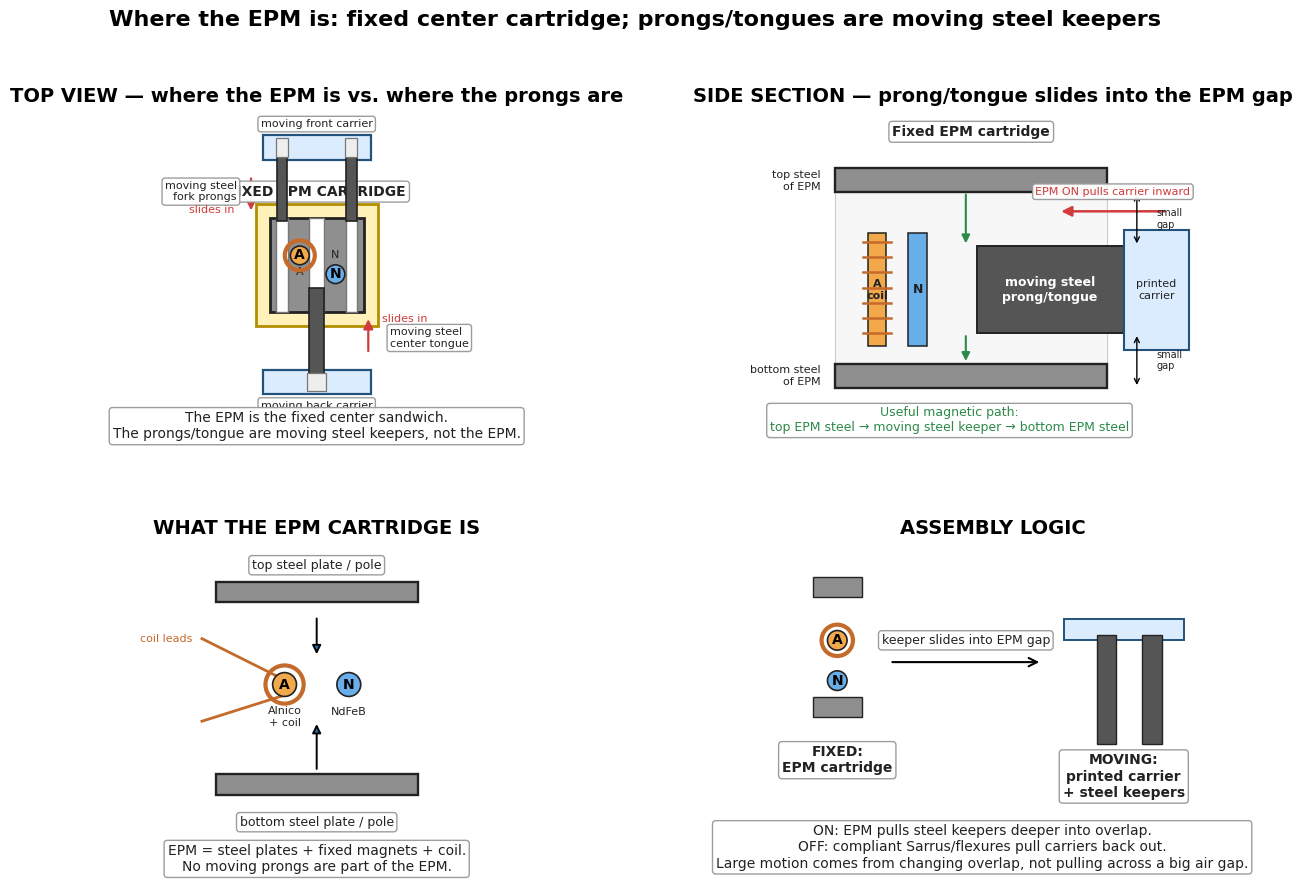
\includegraphics[width=\linewidth]{fixed-cartridge.png}
  \caption{\textbf{Fixed cartridge and moving keeper concept.} The EPM cartridge remains fixed while fork prongs and a center tongue move through the working gap. The useful magnetic path is top pole plate to moving steel keeper to bottom pole plate. This converts the first proof from a broad soft-robot problem into a bench-checkable overlap problem. Source: FluxCell uploaded design figure, 13 May 2026.}
  \label{fig:cartridge}
\end{figure}

\subsection{The lane layout removes collision before it asks for fabrication polish}

The one-axis layer uses a clear comb/fork topology (Fig.~\ref{fig:lane}). The center tongue enters between the Alnico and NdFeB rods, while the fork prongs pass outside the pair. The moving steel pieces therefore interdigitate instead of colliding. This is the key design decision that makes the one-axis proof worth building: the geometry answers the immediate mechanical feasibility question before committing to a monolithic two-axis print.

\begin{figure}[H]
  \centering
  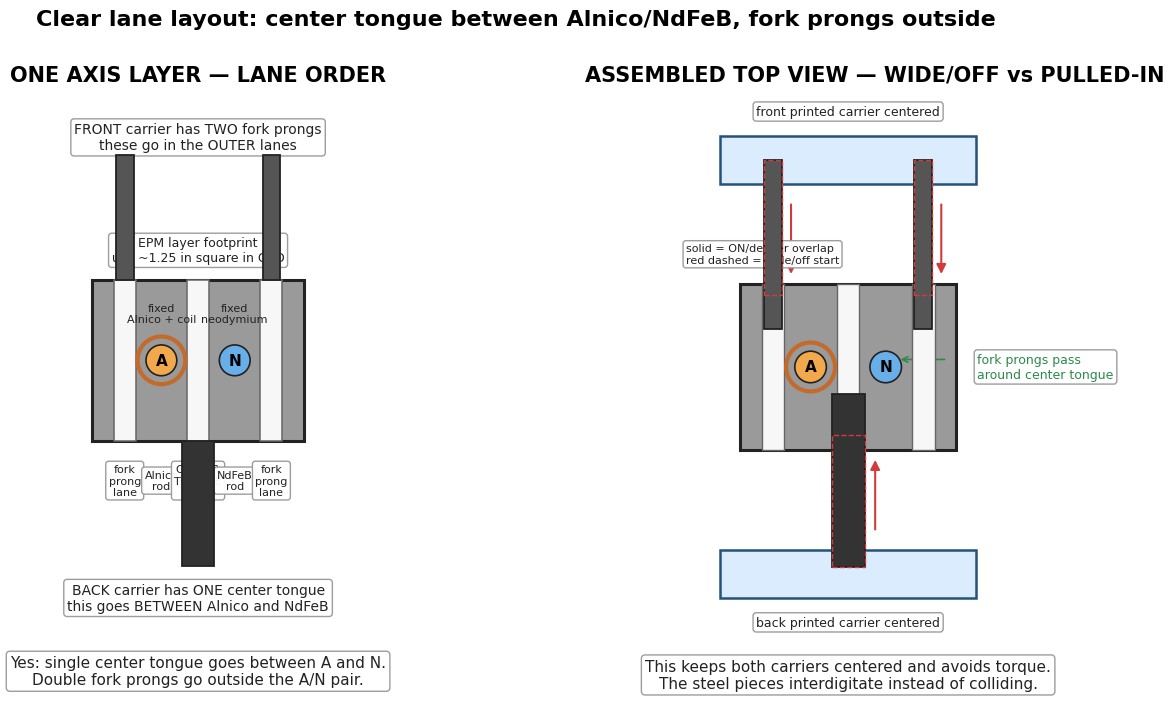
\includegraphics[width=0.92\linewidth]{lane-layout.png}
  \caption{\textbf{Comb/fork lane order.} The center tongue runs between the Alnico and NdFeB positions, and fork prongs run on the outside lanes. The layout keeps both carriers centered and gives the magnetic circuit a repeatable overlap variable. Source: FluxCell uploaded design figure, 13 May 2026.}
  \label{fig:lane}
\end{figure}

\subsection{The current dimensional lock creates a measurable binary proof}

The present dimensional correction uses 1.00 inch keeper inserts rather than 1-1/8 inch inserts. With 1.25 inch square pole plates, the one-axis proof targets a 3.0 inch expanded/off width and a 1.5 inch contracted/on width, corresponding to a 0.75 inch side stroke. The off-state overlap is approximately 0.125 inch and the on-state overlap is approximately 0.875 inch (Fig.~\ref{fig:overlap}). The important experimental consequence is that the proof can be judged by one synchronized record: video of width, current pulse, polarity, hold state, release state, and coil temperature note.

\begin{figure}[H]
  \centering
  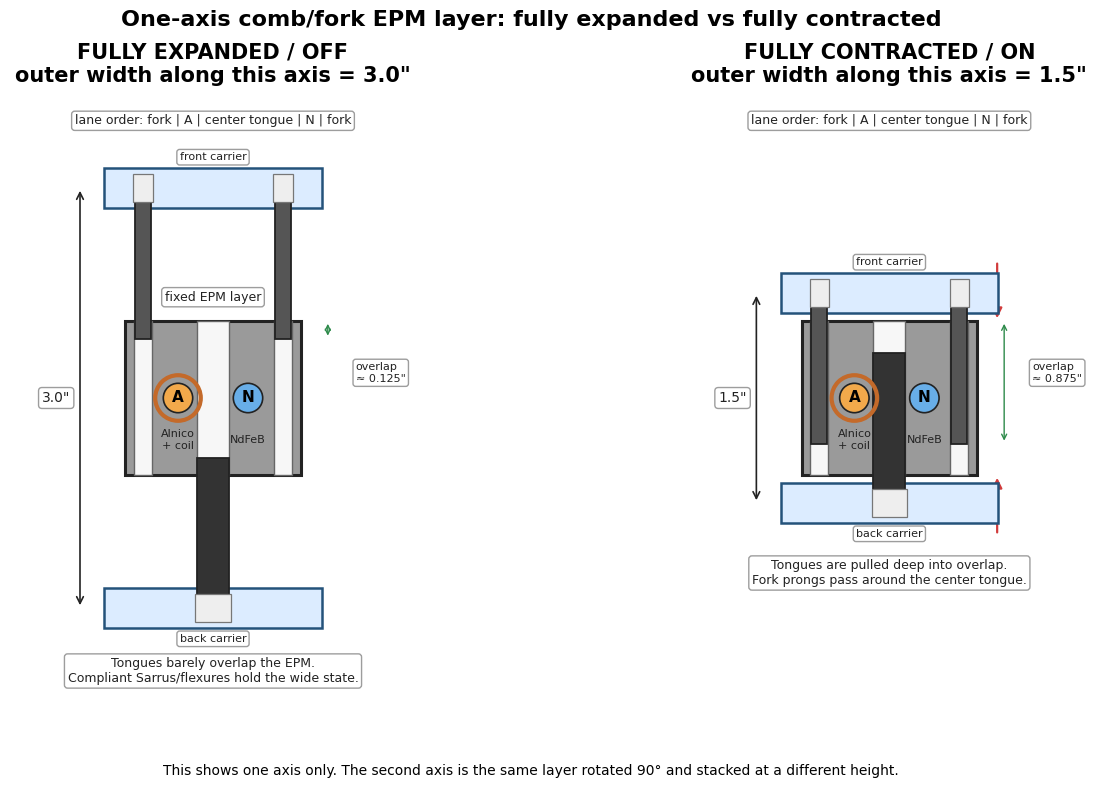
\includegraphics[width=0.86\linewidth]{one-axis-overlap.png}
  \caption{\textbf{One-axis overlap target.} The expanded/off and contracted/on states create a large visible width change while the magnetic variable stays local to keeper overlap. Current evidence locks the geometry; measured force, current, heat, repeatability, and release margins remain pending until the proof is built. Source: FluxCell uploaded design figure, 13 May 2026.}
  \label{fig:overlap}
\end{figure}

\subsection{The build lock is small enough to buy, test, and scale}

\begin{table}[H]
\centering
\small
\caption{\textbf{Locked purchase logic.} The design uses supplier-cut steel dimensions, not home-cut steel, and buys enough for one proof plus four two-axis cells.}
\label{tab:purchase}
\begin{tabular}{>{\raggedright\arraybackslash}p{0.18\linewidth} >{\raggedleft\arraybackslash}p{0.06\linewidth} >{\raggedright\arraybackslash}p{0.49\linewidth} >{\raggedleft\arraybackslash}p{0.11\linewidth}}
\toprule
Part & Qty & Locked specification & Approx total \\
\midrule
Alnico 5 rods & 12 & 0.250 inch diameter by 0.625 inch long, axial & \$23.88 \\
NdFeB rods & 12 & K\&J D4A, 1/4 inch diameter by 5/8 inch long, N42 axial & \(\sim\)\$15.00 \\
Square pole plates & 16 & 1018 steel, 0.25 inch thick by 1.25 inch wide, cut length 1.25 inch & \(\sim\)\$56.00 \\
Fork prong inserts & 24 & A36 flat bar, 1/8 inch by 1/2 inch, cut length 1.00 inch & \$167.28 \\
Center tongue inserts & 12 & 1018 flat bar, 1/4 inch by 1/2 inch, cut length 1.00 inch & \$87.72 \\
Wire, tape, supply, leads, pigtails, heat shrink & set & 30 AWG magnet wire, Kapton, 0--30 V / 0--10 A supply, leads, silicone wire, strain relief & \(\sim\)\$106.75 \\
\bottomrule
\end{tabular}
\end{table}

The total before shipping and tax is approximately \$456.65. This number is not a performance claim. It is a friction claim: the project has a specific, ordered build path and no longer depends on an abstract ``find parts later'' step.

\section{Discussion}

\subsection{Why this could be a strong paper}

The strongest version of this work is not a generic magnetic soft-robot paper. It is a paper about \emph{pulse-programmed mechanical memory}. That framing gives the project a sharper contribution than a one-off actuator: a cell can be addressed briefly, settle into a stable mechanical state, and then become part of a larger surface or body. If the one-axis proof records a clean current pulse, visible width change, zero-current hold, reverse-pulse release, and bounded temperature rise, the manuscript gains the kind of evidence that selective venues can inspect directly.

The paper should stay strict. It should not claim force density, endurance, safety, or scalability until those numbers exist. The current draft therefore marks the bridge from design to evidence: Figure~\ref{fig:cartridge} establishes magnetic architecture, Figure~\ref{fig:lane} establishes collision-free lane logic, Figure~\ref{fig:overlap} establishes the measurable binary state, and Table~\ref{tab:purchase} establishes the build path. The first decisive experiment is not a complete robot. It is the smallest physical demonstration that can falsify or support the mechanism.

\subsection{R\&D and Imagineering relevance}

For an R\&D portfolio aimed at physical experience design, including Disney Imagineering-style work, the compelling story is a quiet kinetic material that remembers shape. A small FluxCell surface could become a visible proof of tangible physical computing: one short pulse changes a body; the body holds without continuous power; the state can be reset; the mechanism is legible on camera; the evidence record includes current, geometry, heat, and repeatability. That combination is closer to show mechanism practice than a purely simulated metamaterial because it foregrounds reliability, inspectability, low standby power, and expressive motion.

The best portfolio concept is a four-cell demonstrator with one choreographed transformation rather than a broad robot. The artifact should show a small surface changing contour or aperture, holding while unplugged, and returning on command. The paper supplies the technical story; the video supplies the human-readable proof.

\subsection{Limitations}

No measured actuation data are claimed in this draft. The current evidence is the design log, uploaded schematic figures, locked dimensions, purchase list, and planned measurement protocol. The main risks are insufficient keeper force, excess friction, heating in the Alnico coil, poor release margin from residual attraction, carrier twist, and fabrication tolerance stack-up. Each risk maps to a first-proof measurement: width trace, current trace, temperature note, hold/release observation, and video from the keeper-gap side.

\section{Materials and Methods}

\subsection{One-axis proof geometry}

The proof uses a fixed center EPM cartridge with two 1.25 inch square pole plates made from 0.25 inch by 1.25 inch 1018 steel rectangle bar cut to 1.25 inch length. The magnetic elements are one 0.250 inch diameter by 0.625 inch long Alnico 5 rod and one 1/4 inch diameter by 5/8 inch long NdFeB rod. The moving keepers are two A36 fork prong inserts, each 1/8 inch by 1/2 inch by 1.00 inch, and one 1018 center tongue insert, 1/4 inch by 1/2 inch by 1.00 inch.

\subsection{Electrical pulse protocol}

The Alnico coil is insulated with Kapton, wound with 30 AWG magnet wire, and connected to an H-bridge driver from a current-limited bench supply. The first test uses short bidirectional pulses separated by zero-drive intervals. For each pulse, the record includes polarity, pulse duration, current limit, observed width, hold state after zero drive, release state after reverse pulse, and a coil temperature note.

\subsection{Acceptance boundary for the first proof}

The first proof succeeds only if the one-axis assembly visibly changes width, holds a state after current returns to zero, releases or reverses under the opposite pulse, and stays within a temperature range safe enough for continued bench testing. A partial result is still useful if it identifies the dominant failure mode: weak magnetic force, high friction, carrier twist, thermal limit, or poor release margin.

\section{Acknowledgements}

This draft was assembled from the FluxCell design log, uploaded ChatGPT-derived geometry figures, and the current locked purchase list.

\section{Funding}

No external funding is claimed in this draft.

\section{Author contributions}

Alan Pham conceived the project direction, maintained the design log, selected the current purchase lock, and defined the proof target. Codex assisted with manuscript drafting, page integration, figure placement, and verification workflow.

\section{Competing interests}

The author declares no competing interests for this draft.

\section{Data availability}

The current data are design records, uploaded schematic figures, supplier links, and purchase specifications. Measured actuation data are pending the one-axis proof.

\section{Code availability}

The current project page, generated proof bundle, and manuscript source are served through the FluxCell site. Arduino pulse code is included in the generated proof bundle.

\section{Additional information}

This is a draft manuscript and design protocol, not a completed experimental report. The claims should be updated after the one-axis proof records measured current, width, temperature, hold, release, and repeatability.

\section{References}
\printbibliography[heading=none]

\end{document}
